\documentclass{standalone}
\usepackage{tikz}
\usetikzlibrary{patterns, positioning}
\usepackage[sfdefault]{ClearSans} %% option 'sfdefault' activates Clear Sans as the default text font
\usepackage[T1]{fontenc}

\begin{document}
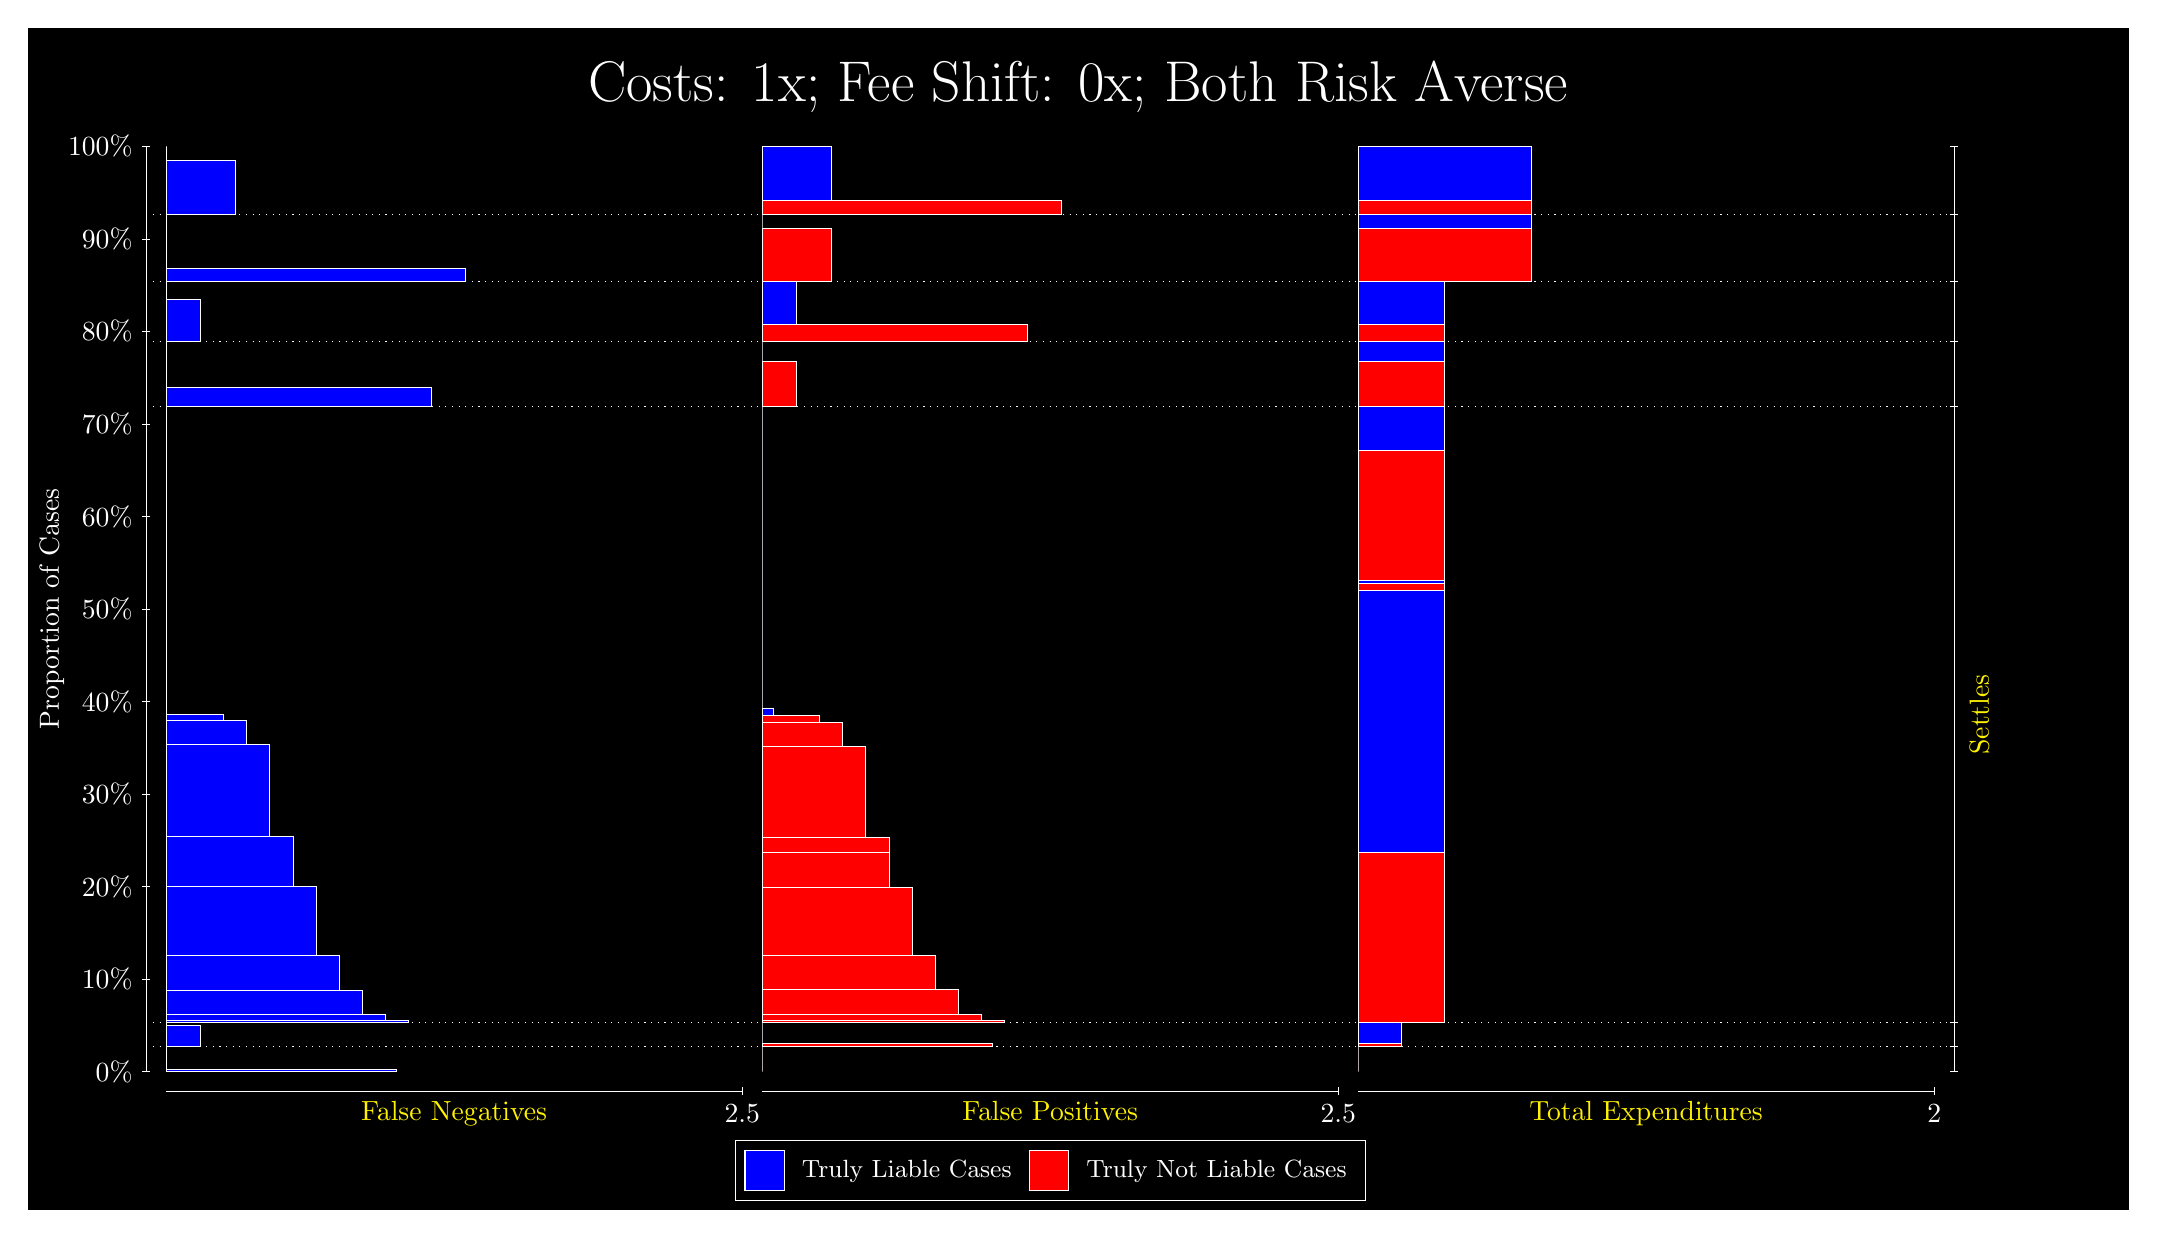
\begin{tikzpicture}
\draw[fill=black] (0,0) rectangle (26.667,15);
\draw[text=white] (0,13.5) rectangle (26.667,15) node[midway] {\huge Costs: 1x; Fee Shift: 0x; Both Risk Averse};
\draw[white, very thin] (1.5,1.75) -- (1.5,13.5);
\node[rotate=90, text=white, anchor=center] at (0.3, 7.625) {Proportion of Cases};
\draw[white, very thin] (1.45,1.75) -- (1.55,1.75);
\node[text=white, anchor=east] at (1.45, 1.75) {0\%};
\draw[white, very thin] (1.45,2.925) -- (1.55,2.925);
\node[text=white, anchor=east] at (1.45, 2.925) {10\%};
\draw[white, very thin] (1.45,4.1) -- (1.55,4.1);
\node[text=white, anchor=east] at (1.45, 4.1) {20\%};
\draw[white, very thin] (1.45,5.275) -- (1.55,5.275);
\node[text=white, anchor=east] at (1.45, 5.275) {30\%};
\draw[white, very thin] (1.45,6.45) -- (1.55,6.45);
\node[text=white, anchor=east] at (1.45, 6.45) {40\%};
\draw[white, very thin] (1.45,7.625) -- (1.55,7.625);
\node[text=white, anchor=east] at (1.45, 7.625) {50\%};
\draw[white, very thin] (1.45,8.8) -- (1.55,8.8);
\node[text=white, anchor=east] at (1.45, 8.8) {60\%};
\draw[white, very thin] (1.45,9.975) -- (1.55,9.975);
\node[text=white, anchor=east] at (1.45, 9.975) {70\%};
\draw[white, very thin] (1.45,11.15) -- (1.55,11.15);
\node[text=white, anchor=east] at (1.45, 11.15) {80\%};
\draw[white, very thin] (1.45,12.325) -- (1.55,12.325);
\node[text=white, anchor=east] at (1.45, 12.325) {90\%};
\draw[white, very thin] (1.45,13.5) -- (1.55,13.5);
\node[text=white, anchor=east] at (1.45, 13.5) {100\%};

\draw[white, very thin] (24.457,1.75) -- (24.457,13.5);
\draw[white, very thin] (24.407,1.75) -- (24.507,1.75);
\node[anchor=west] at (24.407, 1.75) {};
\draw[white, very thin] (24.407,2.0722) -- (24.507,2.0722);
\node[anchor=west] at (24.407, 2.0722) {};
\draw[white, very thin] (24.407,2.3714) -- (24.507,2.3714);
\node[anchor=west] at (24.407, 2.3714) {};
\draw[white, very thin] (24.407,10.2) -- (24.507,10.2);
\node[anchor=west] at (24.407, 10.2) {};
\draw[white, very thin] (24.407,11.02) -- (24.507,11.02);
\node[anchor=west] at (24.407, 11.02) {};
\draw[white, very thin] (24.407,11.783) -- (24.507,11.783);
\node[anchor=west] at (24.407, 11.783) {};
\draw[white, very thin] (24.407,12.637) -- (24.507,12.637);
\node[anchor=west] at (24.407, 12.637) {};
\draw[white, very thin] (24.407,13.5) -- (24.507,13.5);
\node[anchor=west] at (24.407, 13.5) {};

\draw[white, very thin, fill=blue] (1.75,1.75) rectangle (4.6775,1.7839);
\draw[white, very thin, fill=red] (1.75,1.7839) rectangle (1.75,2.0722);
\draw[white, very thin, fill=blue] (1.75,2.0722) rectangle (2.1891,2.34);
\draw[white, very thin, fill=red] (1.75,2.34) rectangle (1.75,2.3714);
\draw[white, very thin, fill=blue] (1.75,2.3714) rectangle (4.8239,2.406);
\draw[white, very thin, fill=blue] (1.75,2.406) rectangle (4.5312,2.4749);
\draw[white, very thin, fill=blue] (1.75,2.4749) rectangle (4.2384,2.7876);
\draw[white, very thin, fill=blue] (1.75,2.7876) rectangle (3.9457,3.2299);
\draw[white, very thin, fill=blue] (1.75,3.2299) rectangle (3.6529,4.1012);
\draw[white, very thin, fill=blue] (1.75,4.1012) rectangle (3.3602,4.7331);
\draw[white, very thin, fill=blue] (1.75,4.7331) rectangle (3.0674,5.9007);
\draw[white, very thin, fill=blue] (1.75,5.9007) rectangle (2.7746,6.2079);
\draw[white, very thin, fill=blue] (1.75,6.2079) rectangle (2.4819,6.2934);
\draw[white, very thin, fill=red] (1.75,6.2934) rectangle (1.75,10.2);
\draw[white, very thin, fill=blue] (1.75,10.2) rectangle (5.1167,10.446);
\draw[white, very thin, fill=red] (1.75,10.446) rectangle (1.75,11.02);
\draw[white, very thin, fill=blue] (1.75,11.02) rectangle (2.1891,11.562);
\draw[white, very thin, fill=red] (1.75,11.562) rectangle (1.75,11.783);
\draw[white, very thin, fill=blue] (1.75,11.783) rectangle (5.5558,11.956);
\draw[white, very thin, fill=red] (1.75,11.956) rectangle (1.75,12.637);
\draw[white, very thin, fill=blue] (1.75,12.637) rectangle (2.6283,13.326);
\draw[white, very thin, fill=red] (1.75,13.326) rectangle (1.75,13.5);
\draw[white, very thin, fill=red] (9.3189,1.75) rectangle (9.3189,2.0383);
\draw[white, very thin, fill=blue] (9.3189,2.0383) rectangle (9.3189,2.0722);
\draw[white, very thin, fill=red] (9.3189,2.0722) rectangle (12.246,2.1036);
\draw[white, very thin, fill=blue] (9.3189,2.1036) rectangle (9.3189,2.3714);
\draw[white, very thin, fill=red] (9.3189,2.3714) rectangle (12.393,2.4052);
\draw[white, very thin, fill=red] (9.3189,2.4052) rectangle (12.1,2.4748);
\draw[white, very thin, fill=red] (9.3189,2.4748) rectangle (11.807,2.7908);
\draw[white, very thin, fill=red] (9.3189,2.7908) rectangle (11.515,3.2231);
\draw[white, very thin, fill=red] (9.3189,3.2231) rectangle (11.222,4.0919);
\draw[white, very thin, fill=red] (9.3189,4.0919) rectangle (10.929,4.5393);
\draw[white, very thin, fill=red] (9.3189,4.5393) rectangle (10.929,4.7285);
\draw[white, very thin, fill=red] (9.3189,4.7285) rectangle (10.636,5.886);
\draw[white, very thin, fill=red] (9.3189,5.886) rectangle (10.344,6.1885);
\draw[white, very thin, fill=red] (9.3189,6.1885) rectangle (10.051,6.2778);
\draw[white, very thin, fill=blue] (9.3189,6.2778) rectangle (9.4652,6.3633);
\draw[white, very thin, fill=blue] (9.3189,6.3633) rectangle (9.3189,10.2);
\draw[white, very thin, fill=red] (9.3189,10.2) rectangle (9.758,10.774);
\draw[white, very thin, fill=blue] (9.3189,10.774) rectangle (9.3189,11.02);
\draw[white, very thin, fill=red] (9.3189,11.02) rectangle (12.686,11.241);
\draw[white, very thin, fill=blue] (9.3189,11.241) rectangle (9.758,11.783);
\draw[white, very thin, fill=red] (9.3189,11.783) rectangle (10.197,12.464);
\draw[white, very thin, fill=blue] (9.3189,12.464) rectangle (9.3189,12.637);
\draw[white, very thin, fill=red] (9.3189,12.637) rectangle (13.125,12.811);
\draw[white, very thin, fill=blue] (9.3189,12.811) rectangle (10.197,13.5);
\draw[white, very thin, fill=red] (16.888,1.75) rectangle (16.888,2.0383);
\draw[white, very thin, fill=blue] (16.888,2.0383) rectangle (16.888,2.0722);
\draw[white, very thin, fill=red] (16.888,2.0722) rectangle (17.437,2.1036);
\draw[white, very thin, fill=blue] (16.888,2.1036) rectangle (17.437,2.3714);
\draw[white, very thin, fill=red] (16.888,2.3714) rectangle (17.986,4.5393);
\draw[white, very thin, fill=blue] (16.888,4.5393) rectangle (17.986,7.8619);
\draw[white, very thin, fill=red] (16.888,7.8619) rectangle (17.986,7.9513);
\draw[white, very thin, fill=blue] (16.888,7.9513) rectangle (17.986,7.9858);
\draw[white, very thin, fill=red] (16.888,7.9858) rectangle (17.986,9.635);
\draw[white, very thin, fill=blue] (16.888,9.635) rectangle (17.986,10.2);
\draw[white, very thin, fill=red] (16.888,10.2) rectangle (17.986,10.774);
\draw[white, very thin, fill=blue] (16.888,10.774) rectangle (17.986,11.02);
\draw[white, very thin, fill=red] (16.888,11.02) rectangle (17.986,11.241);
\draw[white, very thin, fill=blue] (16.888,11.241) rectangle (17.986,11.783);
\draw[white, very thin, fill=red] (16.888,11.783) rectangle (19.083,12.464);
\draw[white, very thin, fill=blue] (16.888,12.464) rectangle (19.083,12.637);
\draw[white, very thin, fill=red] (16.888,12.637) rectangle (19.083,12.811);
\draw[white, very thin, fill=blue] (16.888,12.811) rectangle (19.083,13.5);
\draw[white, dotted] (1.5,2.0722) -- (24.457,2.0722);
\draw[white, dotted] (1.5,2.3714) -- (24.457,2.3714);
\draw[white, dotted] (1.5,10.2) -- (24.457,10.2);
\draw[white, dotted] (1.5,11.02) -- (24.457,11.02);
\draw[white, dotted] (1.5,11.783) -- (24.457,11.783);
\draw[white, dotted] (1.5,12.637) -- (24.457,12.637);
\draw[white, very thin] (1.75,1.5) -- (9.0689,1.5);
\node[text=yellow, anchor=north] at (5.4094, 1.5) {False Negatives};
\draw[white, very thin] (9.0689,1.45) -- (9.0689,1.55);
\node[text=white, anchor=north] at (9.0689, 1.45) {2.5};

\draw[white, very thin] (9.3189,1.5) -- (16.638,1.5);
\node[text=yellow, anchor=north] at (12.978, 1.5) {False Positives};
\draw[white, very thin] (16.638,1.45) -- (16.638,1.55);
\node[text=white, anchor=north] at (16.638, 1.45) {2.5};

\draw[white, very thin] (16.888,1.5) -- (24.207,1.5);
\node[text=yellow, anchor=north] at (20.547, 1.5) {Total Expenditures};
\draw[white, very thin] (24.207,1.45) -- (24.207,1.55);
\node[text=white, anchor=north] at (24.207, 1.45) {2};



\node[text=yellow, centered, rotate=90] at (24.777, 6.2856) {Settles};





\draw (12.978300999999998,1.5) node[draw=none] (baseCoordinate) {};
\begin{scope}[align=center]
        \matrix[scale=0.5, draw=white, below=0.5cm of baseCoordinate, nodes={draw}, column sep=0.1cm]{
            \node[rectangle, draw, minimum width=0.5cm, minimum height=0.5cm, fill=blue] {}; &
            \node[draw=none, font=\small, text=white] (B) {Truly Liable Cases}; &
            \node[rectangle, draw, minimum width=0.5cm, minimum height=0.5cm, fill=red] {}; &
            \node[draw=none, font=\small, text=white] (B) {Truly Not Liable Cases}; \\
            };
\end{scope}

\end{tikzpicture}
\end{document}